\clearpage
\section{Use \noindent Case Modelling}
	
		\subsection{ Based on your domain model create scenarios by modeling the main use \noindent Cases
			and actors as one or more UML use \noindent Case diagram.}
		
			\noindent Case \#1:\\
			(floorplan import)
			importing a background image into the application to be a floorplan\\
			
			
			\noindent Case \#2:\\
			(floorplan export)
			exporting a plan with all the furnitures inside\\
			
			
			\noindent Case \#3:\\
			(catalogue extension)
			importing an image into the application to be a furniture\\
			
			
			\noindent Case \#4:\\
			(catalogue extension)
			drawing in the application to be a furniture\\
			
			
			\noindent Case \#5:\\
			(floorplan, provide information)
			the size of the flat, free vs occupied space, and in-depth info on that\\
			
			
			\noindent Case \#6:\\
			(floorplan validation)
			constraints and rules are applied to check if the arrangement is logically and physically sound\\
			
			
			\noindent Case \#7:\\
			(SSO Login Features)
			in order to allow users to login to our social platform, they are allowed to login via other respected accounts such as Gmail and Facebook\\
			SSO = single-sign-on\\
			
			\noindent Case \#8:\\
			(user, comment)
			users should be allowed to comment on the other published projects\\
			
			
			\noindent Case \#9:\\
			(content moderation)
			user-generated contents have to be inspected before they are allowed to publish (the uploader can see the upload on our website, but others would not until an admin approves the content)
			sub\noindent Cases:\\ floor related (copyright or inappropriate designs), comment-related (laws of speech, inappropriate context)\\
			
			
			\noindent Case \#10:\\
			(user, design)
			users should be allowed to rotate and move furnitures inside a floorplan\\
		
		
		
		\subsection{Use the tabular textual description template uploaded in the exercise materials
			to detail the use \noindent Cases you have identified.}
		
		\clearpage	
		
			Use Case \#1:
			
			\begin{table}[H]
				\scalebox{1.0}{
				\begin{tabularx}{\textwidth}{|l|X|}
					\hline
					Title & floorplan import from image file\\
					\hline
					Primary actor& user\\
					\hline
					Secondary& none\\
					 actor(s)& \\
					 
					\hline
					Goal& having the image plan in  the form that can be used in our application imported from an image\\
					\hline
					Short description& user should be able to use an image of hers as an input for a floorplan, which would be interpreted and recreated as a floorplan structure that can be used in floorplan and furniture arrangement\\
					\hline
					Trigger& click of the user on the button "Submit Image as Floorplan" displayed on the web interface\\
					\hline
					Preconditions&  
						\begin{tabular}[l]{@{}c@{}}
							1) user should browse and select a file from her computer.\\
							2) the file should be in compatible type (JPEG, PNG, BMP)
						\end{tabular}
						\\
					\hline
					Postconditions & None.\\
					\hline
					Main Flow& 
						\begin{tabular}[x]{@{}l@{}}
							1) User selects "Import" tool.\\
							2) Using "Browse" button, user finds the image file that would be imported.\\
							3) User clicks "Submit Image as Floorplan" button.\\
							4) The file is sent via PUSH (HTTP command) to the application server.\\
							5) Application server checks if the sent file is valid file.\\
							5a) if so, the application would convert it to a format that is possible\\
							 to process via the application itself.\\
							6) User is notified about the outcome of the process.
						\end{tabular}
					\\
					\hline
					Additional information & The sent image file size should not exceed 10 MB.\\
					\hline
					Deviation Flows & \\
					\hline
					Deviation Flow 1 & 
						\begin{tabular}[x]{@{}l@{}}
							(earlier steps same as before)\\
							5) Application server checks if the sent file is valid file.\\
							5b) file is either invalid or it is not possible to convert it to a floorplan.\\
							6) User is notified with the information on the image that it is\\
							 not valid.
						\end{tabular}\\
					
					\hline
					Additional Information& \\
					\hline
				\end{tabularx}
				}
			\end{table}
			
			% EXAMPLE USE CASE TABLE
			Use Case \#2:
			\begin{table}[H]
				\scalebox{1.0}{
				\begin{tabularx}{\textwidth}{|l|X|}
					\hline
					Title & floorplan export\\
					\hline
					Primary actor& user\\
					\hline
					Secondary& none\\
					actor(s)& \\
					
					\hline
					Goal& exporting a plan with all the furnitures inside in a format that can be later imported\\
					\hline
					Short description& A user can export one of his projects, or other peoples' projects into a format that can be imported to the application later.\\
					\hline
					Trigger& click of the user on the button "Export Floorplan" displayed on the web interface\\
					\hline
					Preconditions&  
					\begin{tabular}[l]{@{}c@{}}
						1) the project has to be the user's own project or a public project.\\
					\end{tabular}
					\\
					\hline
					Postconditions & None.\\
					\hline
					Main Flow& 
					\begin{tabular}[x]{@{}l@{}}
						1) User navigates to a project via her web browser.\\
						2) User clicks on the "Export Floorplan" button on the respective \\
						webpage\\
						3) The application runs in the server to convert the floorplan with all\\
						 the details into a text file, with necessary additional files if needed, and \\
						 zips them.\\
						4) The application sends the zip file to the user's web client.\\
					\end{tabular}
					\\
					\hline
					Additional information & \\
					\hline
					Deviation Flows & \\
					\hline
					Deviation Flow 1 & 
					\begin{tabular}[x]{@{}l@{}}
						1) User navigates to a project link in which she has no privilege to \\
						display.\\
						2) System does not allow displaying and exporting of the project, \\
						and inform the user about this issue.\\
						
					\end{tabular}\\
					
					\hline
					Additional Information& \\
					\hline
				\end{tabularx}
				}
			\end{table}
		
			\clearpage
		
			Use Case \#3:
			\begin{table}[H]
				\scalebox{1.0}{
				\begin{tabularx}{\textwidth}{|l|X|}
					\hline
					Title &furniture importing via image file\\
					\hline
					Primary actor& user\\
					\hline
					Secondary& none\\
					actor(s)& \\
					
					\hline
					Goal&allowing user to add her own images of furniture to the system\\
					\hline
					Short description& User can take a picture of the furniture she wants to use to arrange her floor, and this picture can be uploaded to the system to be used in our application.\\
					\hline
					Trigger& click of the user on the button "Submit Image as Furniture" displayed on the web interface\\
					\hline
					Preconditions&  
					\begin{tabular}[l]{@{}c@{}}
						None
					\end{tabular}
					\\
					\hline
					Postconditions & None.\\
					\hline
					Main Flow& 
					\begin{tabular}[x]{@{}l@{}}
						1) User navigates to a project of hers.\\
						2) On the project page, she chooses "Import Tools".\\
						3) On the Import Tools menu, she browses and selects one image she \\
						wants to upload.\\
						4) User clicks on the button "Submit Image as Furniture" displayed on \\
						the web interface\\
						5) The file is sent via PUSH (HTTP command) to the application server.\\
						6) Application server checks if the sent file is valid file.\\
						6a) if so, the system informs the user on the positive outcome.
					\end{tabular}
					\\
					\hline
					Additional information & The sent file size should not exceed 10 MB. \\
					\hline
					Deviation Flows & \\
					\hline
					Deviation Flow 1 & 
					\begin{tabular}[x]{@{}l@{}}
						(previous steps same as before)\\
						6b) if not valid, then the system would inform the user about the\\
						 negative outcome.\\
					\end{tabular}\\
					
					\hline
					Additional Information& \\
					\hline
				\end{tabularx}
				}
			\end{table}
		
			Use Case \#4:
			\begin{table}[H]
				\scalebox{1.0}{
				\begin{tabularx}{\textwidth}{|l|X|}
					\hline
					Title & Drawing a Furniture\\
					\hline
					Primary actor& user\\
					\hline
					Secondary& none\\
					actor(s)& \\
					
					\hline
					Goal& Allowing user to draw sketches that are to be converted into furnitures to be used in the application\\
					\hline
					Short description& Using the website of the application, a user can draw a furniture. After the drawing is finalized, user can opt to convert the drawing into a furniture she can use in the future.\\
					\hline
					Trigger& \\
					\hline
					Preconditions&  
					\begin{tabular}[l]{@{}c@{}}
						None
					\end{tabular}
					\\
					\hline
					Postconditions & None.\\
					\hline
					Main Flow& 
					\begin{tabular}[x]{@{}l@{}}
						1) User navigates to the "Drawing" page. \\
						2) User draws a furniture on her own imagination.\\
						3) User finalizes drawing.\\
						4) After saving, user is asked whether she wants to convert the\\
						 drawing into a furniture.\\
						5a) If positively answered, the drawing would be converted into a \\
						furniture, and would be added to the user's library.\\
						6) The user would be informed on the outcome of the conversion, and \\
						also about where the new furniture can be accessed.
					\end{tabular}
					\\
					\hline
					Additional information & \\
					\hline
					Deviation Flows & \\
					\hline
					Deviation Flow 1 & 
					\begin{tabular}[x]{@{}l@{}}
						(previous steps same as before)\\
						
						5b) if negatively answered, the drawing will be stored as it is, \\
						it won't be converted into a furniture.
						
					\end{tabular}\\
					
					\hline
					Additional Information& \\
					\hline
				\end{tabularx}
				}
			\end{table}
			
			\clearpage
		
			Use Case \#5:
			\begin{table}[H]
				\scalebox{1.0}{
				\begin{tabularx}{\textwidth}{|l|X|}
					\hline
					Title & provision of information about a floorplan\\
					\hline
					Primary actor& user\\
					\hline
					Secondary& none\\
					actor(s)& \\
					
					\hline
					Goal& to provide a user information about a flat\\
					\hline
					Short description& the size of the flat, free space, space occupied by furniture has to be provided to a user.\\
					\hline
					Trigger& A change in the layout of the floor\\
					\hline
					Preconditions&   
					\begin{tabular}[l]{@{}c@{}}
						None
					\end{tabular}
					\\
					\hline
					Postconditions & None.\\
					\hline
					Main Flow& 
					\begin{tabular}[x]{@{}l@{}}
						1) User navigates to the view of the floorplan.\\
						2) The said info about the floor is displayed on the GUI.\\
						3) Whenever a change is applied to the layout of the floor by user \\
						(moving of the furniture, addition or removal of the furniture, change in \\
						the floor properties, etc.), those information is recalculated on the\\
						 client-side.\\
						4) After the calculation, the GUI is updated to reflect the changes.\\
					\end{tabular}
					\\
					\hline
					Additional information & \\
					\hline
					Deviation Flows &  (there is none)\\
					\hline
				\end{tabularx}
				}
			\end{table}
		
			Use Case \#6:
			\begin{table}[H]
				\scalebox{1.0}{
				\begin{tabularx}{\textwidth}{|l|X|}
					\hline
					Title & Checking of the Constraints and Rules on a Floorplan\\
					\hline
					Primary actor& user\\
					\hline
					Secondary& none\\
					actor(s)& \\
					
					\hline
					Goal& to check whether the current state of a floorplan is logically and physically sound\\
					\hline
					Short description& Checking physical limits of the layout is needed to see whether such arrangement is possible.\\
					\hline
					Trigger& A change in the layout of the floor\\
					\hline
					Preconditions&  
					\begin{tabular}[l]{@{}c@{}}
						None.
					\end{tabular}
					\\
					\hline
					Postconditions & None.\\
					\hline
					Main Flow& 
					\begin{tabular}[x]{@{}l@{}}
						1) User navigates to the view of the floorplan.\\
						2) Whenever a change is applied to the layout of the floor by user \\
						(moving of the furniture, addition or removal of the furniture, change in \\
						the floor properties, etc.), the sanity check is performed on the server.\\
						3a) If the submitted layout is sound, client application is informed that \\
						the change is alright, and it is safe to continue.
					\end{tabular}
					\\
					\hline
					Additional information & \\
					\hline
					Deviation Flows & \\
					\hline
					Deviation Flow 1 & 
					\begin{tabular}[x]{@{}l@{}}
						(previous steps same as before)\\
						3b) If the submitted layout is not sound, client application is informed \\
						that the change is not alright.\\
						4) Client application reverts back the last change, and informs user \\
						that the action is not performable.
					\end{tabular}\\
					
					\hline
					Additional Information& \\
					\hline
				\end{tabularx}
				}
			\end{table}

			\clearpage
		
			Use Case \#7:
			\begin{table}[H]
				\scalebox{1.0}{
				\begin{tabularx}{\textwidth}{|l|X|}
					\hline
					Title & SSO Login\\
					\hline
					Primary actor& user\\
					\hline
					Secondary& none\\
					actor(s)& \\
					
					\hline
					Goal& to allow users login with their respectable service accounts\\
					\hline
					Short description& for ease of use, users should be allowed to login to our system using their respectable online accounts such as Facebook and Google accounts \\
					\hline
					Trigger& click on the buttons such as "Login with Facebook" and ""Login with Google\\
					\hline
					Preconditions&  
					\begin{tabular}[l]{@{}c@{}}
						None
					\end{tabular}
					\\
					\hline
					Postconditions & None.\\
					\hline
					Main Flow& 
					\begin{tabular}[x]{@{}l@{}}
						1) user navigates to the login page\\
						2) instead of creating a new account from scratch, user selects one of two buttons\\
						3) in case of Google, we call the Google single-sign-on webpage\\
						4) user fills in her details\\
						5a) Google passes a token to our server. \\
						6) User is both signed up and signed in at the same time.\\
						7) User client is redirected to her home page of our website.
					\end{tabular}
					\\
					\hline
					Additional information & There exists deviations for Facebook login, but just the service provider name changes, all the steps are the same. \\
					\hline
					Deviation Flows & \\
					\hline
					Deviation Flow 1 & 
					\begin{tabular}[x]{@{}l@{}}
						(previous steps same as usual)\\
						5b) User fails to login, so Google passes a message saying the login has failed.\\
						6) User is informed that login is failed, so she can try again.\\
						
					\end{tabular}\\
					
					\hline
					Additional Information& \\
					\hline
				\end{tabularx}
				}
			\end{table}

			Use Case \#8:
			\begin{table}[H]
				\scalebox{1.0}{
				\begin{tabularx}{\textwidth}{|l|X|}
					\hline
					Title & commenting on contents\\
					\hline
					Primary actor& user\\
					\hline
					Secondary& moderator(s)\\
					actor(s)& \\
					
					\hline
					Goal& to enable user to comment on the projects (floorplans and furnitures)\\
					\hline
					Short description& as one requirement in the assignment body dictates, the users should be allowed to comment on each others' projects.\\
					\hline
					Trigger& clicking on the button "Send Comment" \\
					\hline
					Preconditions&  
					\begin{tabular}[l]{@{}l@{}}
						1) text field of the comment should be not empty.\\
						2) text field should not contain any banned words (offensive, racist, etc.)
					\end{tabular}
					\\
					\hline
					Postconditions & None.\\
					\hline
					Main Flow& 
					\begin{tabular}[x]{@{}l@{}}
						1) user navigates to a project page.\\
						2) user fills in the text field.\\
						3) user clicks "Send Comment" button.\\
						4) the comment is sent to the application server via POST command.\\
						5) the application server checks for banned words.\\
						6a) if it does not contain any banned words, it is stored for approval of a moderator.\\
						7a) after moderation is done, and approval is given, the post is made visible on the said project. 
					\end{tabular}
					\\
					\hline
					Additional information & \\
					\hline
					Deviation Flows & \\
					\hline
					Deviation Flow 1 & 
					\begin{tabular}[x]{@{}l@{}}
						6b) if it does contain at least one banned words, it is directly discarded,\\
						and user is informed about the situation.\\
						
					\end{tabular}\\
					
					\hline
					Deviation Flow 2 & 
					\begin{tabular}[x]{@{}l@{}}
						7b) if it does not granted the approval of a moderator, it is deleted,\\
						and user is informed about the situation.\\
						
					\end{tabular}\\
					
					\hline
					Additional Information& \\
					\hline
				\end{tabularx}
				}
			\end{table}
		
			\clearpage
		
			Use Case \#9:
			\begin{table}[H]
				\scalebox{1.0}{
				\begin{tabularx}{\textwidth}{|l|X|}
					\hline
					Title & moderation of contents\\
					\hline
					Primary actor& moderator(s)\\
					\hline
					Secondary& none\\
					actor(s)& \\
					
					\hline
					Goal& to not allow any illegal or offensive content to be stored on the service\\
					\hline
					Short description& to be lawful, and to not get into trouble with copyrights and patents, the user-created content has to be inspected.\\
					\hline
					Trigger& a moderator clicking on an item that lies in the "User Content Waiting for Approval" page\\
					\hline
					Preconditions&  
					\begin{tabular}[l]{@{}c@{}}
						None 
					\end{tabular}
					\\
					\hline
					Postconditions & None.\\
					\hline
					Main Flow& 
					\begin{tabular}[x]{@{}l@{}}
						1) a moderator navigates to the "User Content Waiting for Approval" page\\
						2) moderator clicks on an item, be it a comment or a user-created content\\
						3) moderator goes over the item, and based on her decision, click the respective\\
						"Accept" or "Reject" button.\\
						4a) in case of accept, the content is made visible to all the users. \\
						5) the user is notified about the approval, stating that the content is approved and \\
						visible to all.\\
					\end{tabular}
					\\
					\hline
					Additional information & \\
					\hline
					Deviation Flows & \\
					\hline
					Deviation Flow 1 & 
					\begin{tabular}[x]{@{}l@{}}
						4b) in case of reject, the content is deleted from the server.\\
						5) the user is notified about the rejection, and the reason why.\\
						
					\end{tabular}\\
					
					\hline
					Additional Information& \\
					\hline
				\end{tabularx}
				}
			\end{table}
		
					\noindent Case \#10:\\
		(user, design)
		users should be allowed to rotate and move furnitures inside a floorplan\\
		
			Use Case \#10:
			\begin{table}[H]
				\scalebox{1.0}{
				\begin{tabularx}{\textwidth}{|l|X|}
					\hline
					Title & arrangement functionality of furnitures\\
					\hline
					Primary actor& user\\
					\hline
					Secondary& none\\
					actor(s)& \\
					
					\hline
					Goal& to allow users to arrange furnitures on a floorplan as their heart desire\\
					\hline
					Short description& user should be able to rotate and move around the furnitures using our service.\\
					\hline
					Trigger& a click on a furniture in the floorplan view\\
					\hline
					Preconditions&  
					\begin{tabular}[l]{@{}c@{}}
						None.
					\end{tabular}
					\\
					\hline
					Postconditions & None.\\
					\hline
					Main Flow& 
					\begin{tabular}[x]{@{}l@{}}
						1) user navigates to a project of hers.\\
						2) user clicks on a furniture\\
						3) a menu appears with affordances such as rotation and move\\
						4) user moves and rotates the furniture around\\
						5) after user finishes moving the said furniture, user clicks on the "Finish" button.\\
						6) the new position and rotation of the furniture is sent to the application server,\\
						 to be checked for constraints (the rest is functionality use case \#6).
					\end{tabular}
					\\
					\hline
					Additional information & \\
					\hline
					Deviation Flows & None\\
					\hline
					
					\hline
					Additional Information& \\
					\hline
				\end{tabularx}
				}
			\end{table}
		
		\clearpage
			
			
		\subsection{In the first step, you should have identified around 10 use Cases. Please specify
			five of these using UML activity diagrams. Do mind, that these should not be
			trivial!}
		
            \noindent Case \#1:
            (Import floorplan from image file)
            
            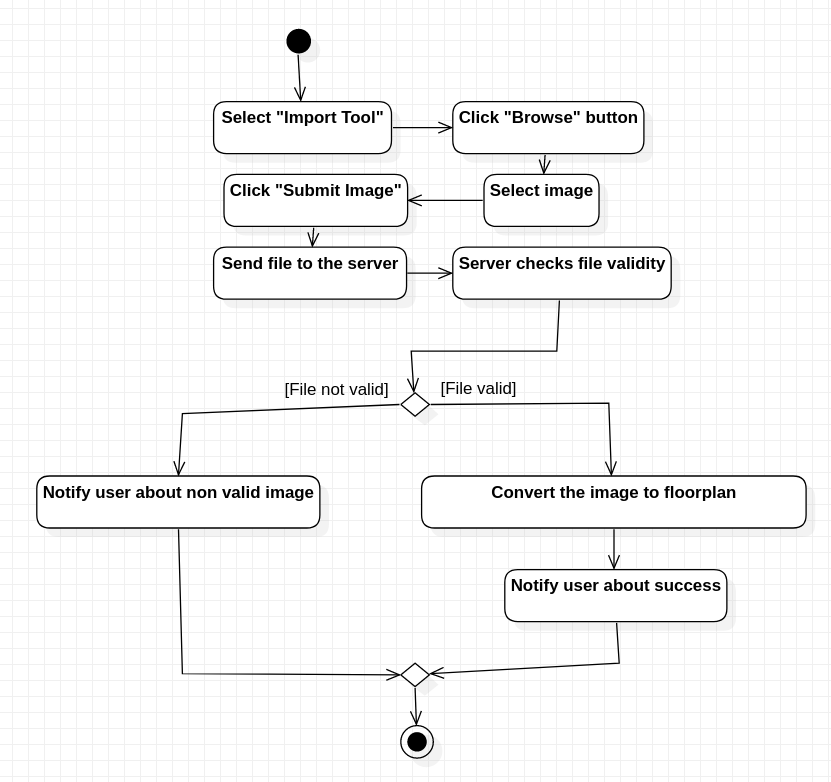
\includegraphics[width=\textwidth]{images/j_UseCase1.png}
        
			\noindent Case \#7:
			(SSO Login Features)
			
			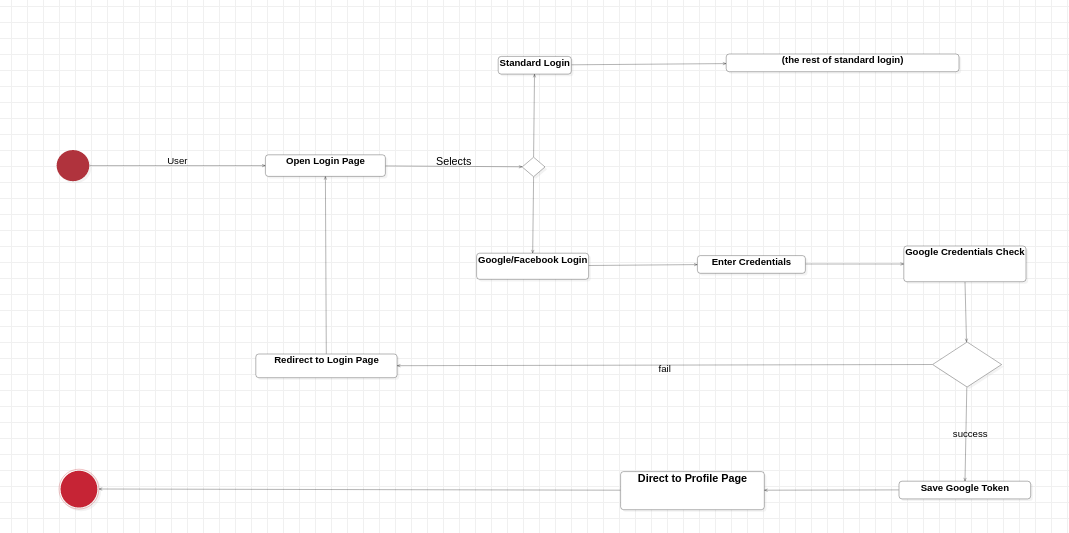
\includegraphics[width=\textwidth]{images/sso.png}
		
	\noindent Case \#8:
	(Comment)
			
	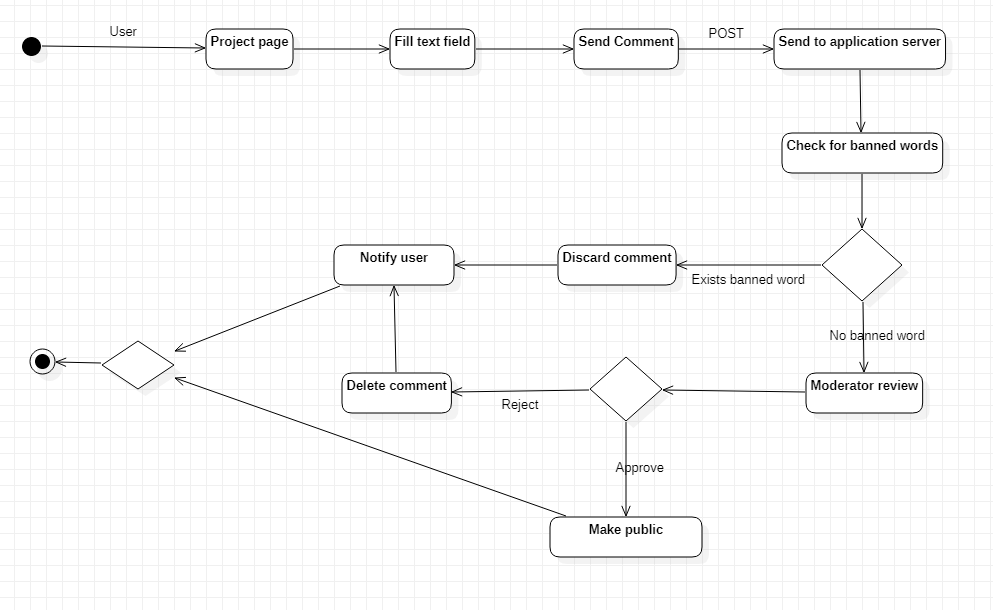
\includegraphics[width=\textwidth]{images/UseCase8_Comment.png}		
		
		\subsection{Explain the advantages of using activity diagrams.}
		
		Although use-case diagrams are helpful for discussing how a system broadly behaves, they are not enough to show the underlying logic. With activity diagrams, a observer can see which component is conveying what kind of information, and how decisions are made.\\
		
		In other words, activity diagrams display also both the positive and negative deviations, and easier to observe than use case diagrams.